\section{Objectives}
\label{sec:objectives}
The life-cycle of a Cloud-based IoT application is composed by several stages,
as illustrated in the Figure \ref{fig:life-cycle}. Some of the stages are placed in
the smart place while others are placed in the Cloud.
% Application Life-cycle
\begin{figure}[h!]
  \centering
  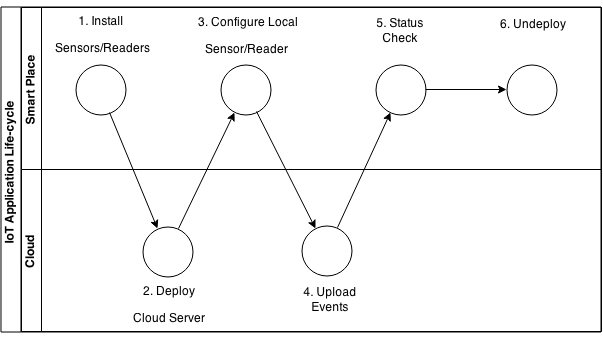
\includegraphics[width=\textwidth]{./images/life-cycle}
  \caption{IoT application life-cycle.}
  \label{fig:life-cycle}
\end{figure}

The life-cycle of an IoT application starts with the installation of the sensors and
readers in the smart place (step 1). The next step consists in preparation to
process the events sent by the smart objects. First the application must be deployed at
the Cloud in order to be able to receive the events (step 2). After that the installed
sensors and readers must be configured to send the generated events to the application that is
running in the Cloud (step 3). At this point the smart place is already configured to
support the processing of events generated by smart objects (step 4). The monitoring of the
the performance of the application in the smart place is performed to determine if the
application is running  with the desired \textit{QoS} (step 5). The final stage that an IoT
application can reach is its undeployment, which means that the smart place is deactivated (step 6).\\

The main objective of Cloud4Things is to decrease the complexity of the deployment of Cloud-based
IoT applications in a smart place. Usually the deployment of such applications require that
all the components of the application are manually configured and installed. In order
to reduce the complexity of this process, Cloud4Things will automate the deployment process
of Cloud-based IoT applications. To automate the deployment process of the applications
Cloud4Things will rely in Cloud Orchestrators tools to execute such operation. These
tools allows the specification of the components and the relation between them in a
high-level abstraction, provisioning the necessary resources at the Cloud in a effective
way and monitoring the application during its life-cycle.\\

However, orchestration tools do not solve all problems. In particular, RFID applications require a
software stack that usually is composed by a database, a web server and the software components
that implements the EPC Network standards. But these tools lack the integration of the EPC
Network software with the other components. Thus, to support the deployment of IoT applications
that are based in RFID technologies, the orchestration tool that will perform the deployment
of the application need to be extend to support the integration of the EPC software components
with the other software components that are required by the application.\\

Another aspect that is important is guarantee that Cloud providers are delivering
the desired service level. As sub objective, Cloud4Things will allow to define the
\textit{QoS} parameters that specify the desired service level through the orchestration
tool. These \textit{QoS} parameters will be expressed in terms of SLAs that will be
negotiated between the Cloud provider and the customer. The definition of these \textit{QoS}
parameters will allow monitoring the performance of the application and verify if the
delivered service level meet with the expectations. In order to monitoring the performance
of the application, Cloud4Things will need to monitor the service delivered by Cloud
providers and determine if the level of this service guarantee an
acceptable \textit{QoS} for the application.
